% !TEX TS-program = pdflatex
% !TEX encoding = UTF-8 Unicode

% This is a simple template for a LaTeX document using the "article" class.
% See "book", "report", "letter" for other types of document.

\documentclass[20pt]{article} % use larger type; default would be 10pt

\usepackage[utf8]{inputenc} % set input encoding (not needed with XeLaTeX)

%%% Examples of Article customizations
% These packages are optional, depending whether you want the features they provide.
% See the LaTeX Companion or other references for full information.

%%% PAGE DIMENSIONS
\usepackage{geometry} % to change the page dimensions
\geometry{a4paper} % or letterpaper (US) or a5paper or....
% \geometry{margin=2in} % for example, change the margins to 2 inches all round
% \geometry{landscape} % set up the page for landscape
%   read geometry.pdf for detailed page layout information

\usepackage{graphicx} % support the \includegraphics command and options

% \usepackage[parfill]{parskip} % Activate to begin paragraphs with an empty line rather than an indent

%%% PACKAGES
\usepackage{booktabs} % for much better looking tables
\usepackage{array} % for better arrays (eg matrices) in maths
\usepackage{paralist} % very flexible & customisable lists (eg. enumerate/itemize, etc.)
\usepackage{verbatim} % adds environment for commenting out blocks of text & for better verbatim
%\usepackage{subfig} % make it possible to include more than one captioned figure/table in a single float
\usepackage{mathtools}
\usepackage{graphicx} % supports images in latex
% These packages are all incorporated in the memoir class to one degree or another...

\usepackage{graphicx}
\usepackage{subcaption}

%%% Other stuff
\DeclarePairedDelimiter\ceil{\lceil}{\rceil}
\DeclarePairedDelimiter\floor{\lfloor}{\rfloor}

%%% HEADERS & FOOTERS
\usepackage{fancyhdr} % This should be set AFTER setting up the page geometry
\pagestyle{fancy} % options: empty , plain , fancy
\renewcommand{\headrulewidth}{0pt} % customise the layout...
\lhead{}\chead{}\rhead{}
\lfoot{}\cfoot{\thepage}\rfoot{}

%%% SECTION TITLE APPEARANCE
\usepackage{sectsty}
\allsectionsfont{\sffamily\mdseries\upshape} % (See the fntguide.pdf for font help)
% (This matches ConTeXt defaults)

%%% ToC (table of contents) APPEARANCE
\usepackage[nottoc,notlof,notlot]{tocbibind} % Put the bibliography in the ToC
\usepackage[titles,subfigure]{tocloft} % Alter the style of the Table of Contents
\renewcommand{\cftsecfont}{\rmfamily\mdseries\upshape}
\renewcommand{\cftsecpagefont}{\rmfamily\mdseries\upshape} % No bold!

%%% graphics path


%%% END Article customizations

%%% nice things to keep around
%\begin{figure}[!htbp]
%  	\centering
%   	\begin{subfigure}[p]{0.5\linewidth}
%    	\includegraphics[width=\linewidth]{}
%   	\end{subfigure}
%\end{figure} 

% \noindent\rule{2cm}{0.4pt} 
%%% puts a small horizontal line

% \mathcal{O} 
%%% big O notation

% \begin{table}
% \caption{Forward slash.}
% \[\begin{array}{c|ccccc} 
% abc/def & 1 & 2 & 3 & 4 & 5\\
% \hline
% 1 & a & b & c & d & e\\
% 2 & f & g & h & i & j\\
% 3 & k & l & m & n & o\\
% \end{array}\]
% \end{table}

%%% The "real" document content comes below...

\title{Formal Languages Homework 5}
\author{Liam Dillingham}
%\date{} % Activate to display a given date or no date (if empty),
         % otherwise the current date is printed 

\begin{document}
\maketitle

\section{Problem 4.1.1}
Prove that the following languages are not regular languages
\subsection{e). $\{0^{n}10^{n} \ \mid \ n\geq1\}$}
Using the pumping lemma, suppose that $x=\epsilon, y=0^{n}$, and $z=10^{n}$.  Note that $|xy| \leq n$, and $y \neq \epsilon$.  However, note that the pumping lemma requires that for all $k \geq 0$, the string is still in our language $L$.  Lets choose $k=0$.  Then the string is essentially $10^{n}$, where the number of 0's on either side of the 1 do not match.  Therefore, the language is not regular.
\subsection{f). $\{0^{n}1^{2n} \ \mid \ n\geq1\}$}
Let $x=\epsilon, y = 0^{n}, z=1^{2n}$. By choosing a $k=0$, we have $0^{n*0}=\epsilon$.  Since the number of 1's is not a square of the number of 0's, the language is not regular.

\section{Problem 4.1.2}
Prove that the following are not regular languages
\subsection{e). The set of strings of 0's and 1's that are of the form $ww$, that is, some string repeated}
Let $x=\epsilon$, and $y=w$, and $z=w$.  Then $yz$ should be in the language. However, by choosing any $k \neq 1$ gives us a string not equal to $ww$, and thus not in the language.  Therefore the language is not regular.

\newpage
\section{Problem 4.2.4}
Which of the following identities are true?
\subsection{a). $(L/a)a=L$ (the left side represents the concatenation of the languages $L/a$ and $\{a\}$)}
Note that $(L/a)$ is the set of words in $L$ such that $wa$ is in $L$.  So if there is a word in $L$ such that it ends in some other symbol, such as $b$, then it will not be in $(L/a)$.  Thus concatentating $a$ again on the end will not restore the set to $L$.  Thus, false.
\subsection{b). $a(a\setminus L)=L$ (again, concatenation with $\{a\}$, this time on the left is intended)}
The argument for this identity follows the same as above, except on the left.  Thus, false.
\subsection{c). $(La)/a=L$}
$(La)$ is the set of all $w \in L$ with an $a$ concatenated on the right side.  And $(La)/a$ is all $w \in L$ where $wa$ is also in $L$.  Since we are appending an $a$ to every $w \in L$, then we take the quotient, where we only keep $w$'s such that they have an $a$ on the right side, then yes, it returns the original $L$. Thus true.
\subsection{d). $a\setminus (aL)=L$}
The argument follows the same from above, except considering for the left side of the $w$'s. Thus true.

\newpage
\section{Problem 4.4.2}
Given the following transition table of a DFA
\begin{figure}[!htbp]
  	\centering
   	\begin{subfigure}[p]{0.15\linewidth}
    	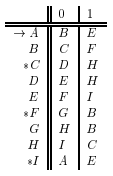
\includegraphics[width=\linewidth]{./figures/HW5fig1.png}
   	\end{subfigure}
\end{figure} 
\subsection{a). Draw the table of distinguishabilities for this automaton}
\begin{figure}[!htbp]
  	\centering
   	\begin{subfigure}[p]{0.4\linewidth}
    	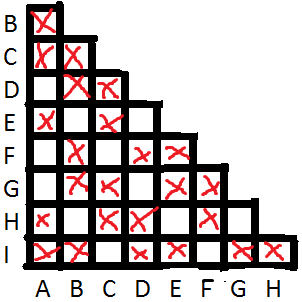
\includegraphics[width=\linewidth]{./figures/h5-1.png}
   	\end{subfigure}
\end{figure} 
\subsection{b). Construct the minimum-state equivalent DFA}
\begin{figure}[!htbp]
  	\centering
   	\begin{subfigure}[p]{0.5\linewidth}
    	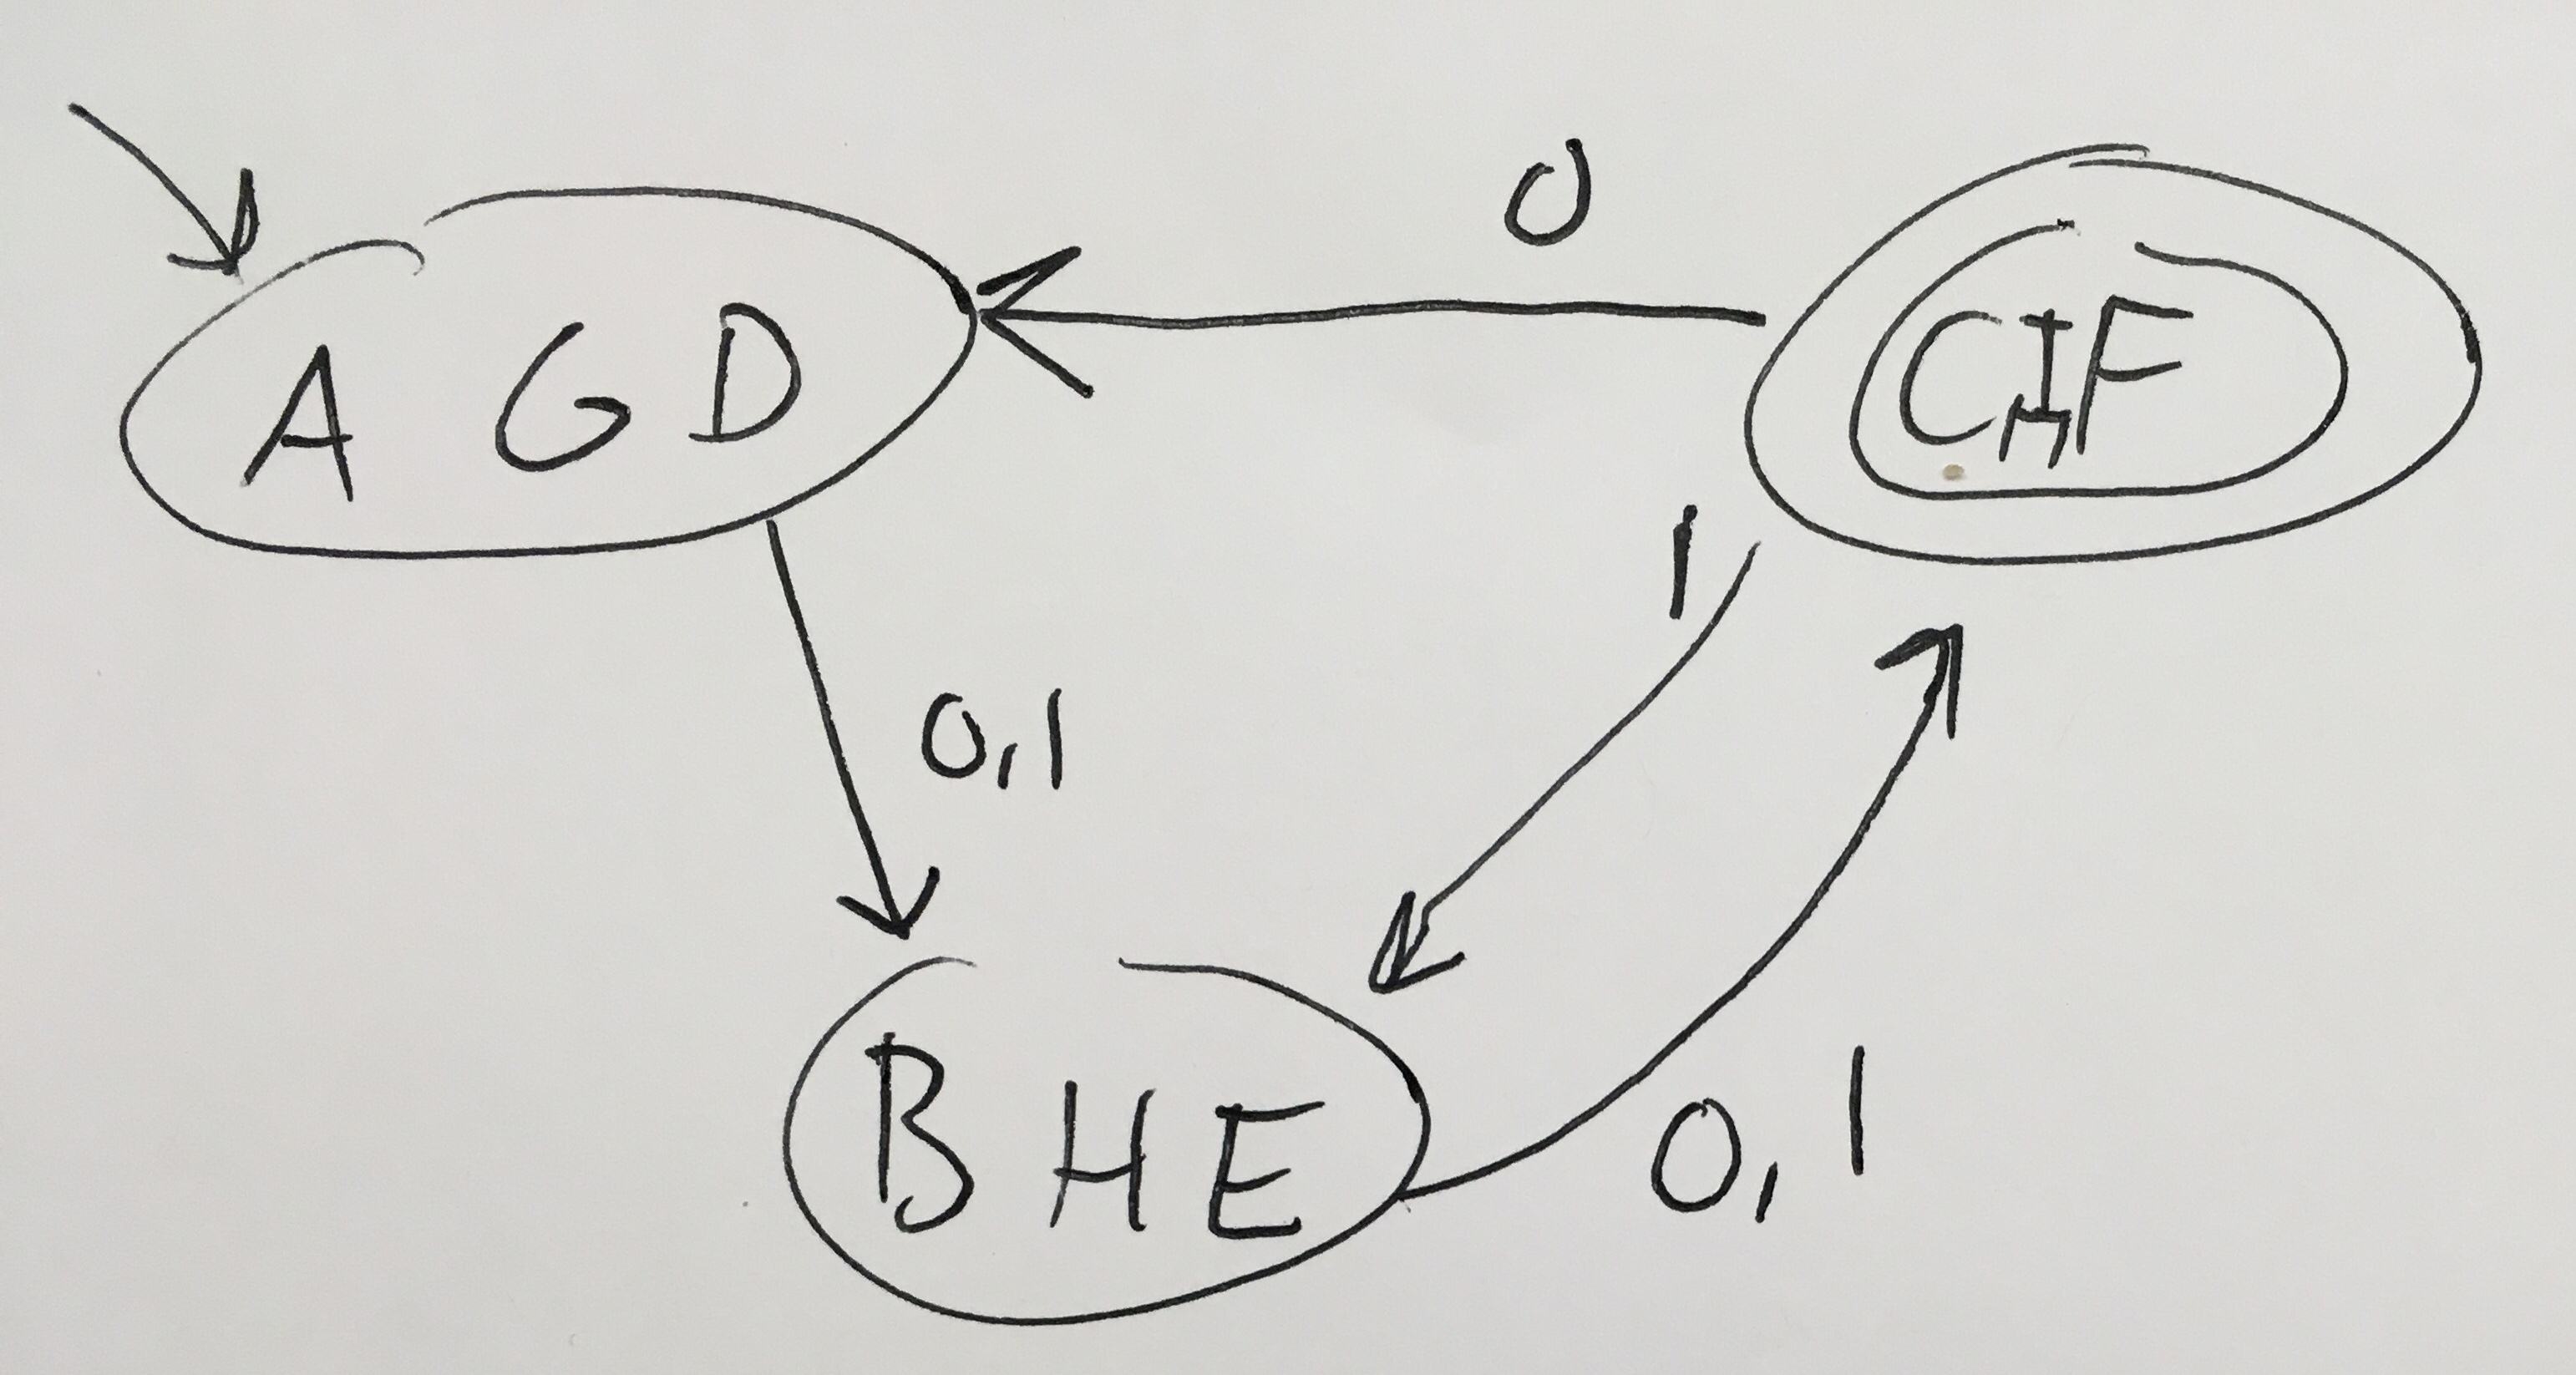
\includegraphics[width=\linewidth]{./figures/h5-2.jpg}
   	\end{subfigure}
\end{figure} 

\end{document}






